\documentclass[conference]{IEEEtran}
\IEEEoverridecommandlockouts
\usepackage{cite}
\usepackage{amsmath,amssymb,amsfonts}
\usepackage{algorithmic}
\usepackage{graphicx}
\usepackage{textcomp}
\usepackage{xcolor}
\usepackage{booktabs}
\usepackage{multirow}
\usepackage{url}
\usepackage{tikz}
\usetikzlibrary{shapes.geometric, arrows.meta, positioning, fit}

\def\BibTeX{{\rm B\kern-.05em{\sc i\kern-.025em b}\kern-.08em
    T\kern-.1667em\lower.7ex\hbox{E}\kern-.125emX}}

\begin{document}

\title{TriGuard: Securing Tool-Augmented LLM Agents Through Provenance-Aware Mediation and Action Verification}

\author{
\IEEEauthorblockN{Irsa Azeem\IEEEauthorrefmark{1}, Muhammad Anas\IEEEauthorrefmark{2}, and Muhammad Wasim\IEEEauthorrefmark{3}}
\IEEEauthorblockA{Department of Computer Science\\
University of Management and Technology\\
Sialkot, Pakistan\\
\IEEEauthorrefmark{1}irsaazeem090@gmail.com \quad
\IEEEauthorrefmark{2}anas1054108@gmail.com \quad
\IEEEauthorrefmark{3}muhammad-wasim@skt.umt.edu.pk}
}

\maketitle

\begin{abstract}
Tool-augmented Large Language Model (LLM) agents are vulnerable to indirect prompt injection (IPI) attacks, in which malicious instructions embedded in external content redirect agents toward unauthorized actions. Existing defenses primarily focus on detecting, filtering, or rewriting malicious inputs, which can induce severe formatting collapse on structured tool outputs, incur multi-second latency overheads, or fail to enforce authorization before physical tool execution. To address this limitation, we propose TriGuard, a training-free, three-tier defense framework integrating capability-based authorization, provenance-aware context mediation, and deterministic intent-consistency verification. TriGuard derives task-specific capability scopes and argument-level constraints (recipient whitelists, canonical file paths, and destination domains) from trusted user instructions, binds them into HMAC-SHA256 tokens, isolates untrusted external content within provenance-tagged boundaries, and validates proposed tool invocations through a default-deny execution gateway with a mean CPU overhead of $128.1~\mu\text{s}$ ($0.13\text{ ms}$) per episode. We evaluate TriGuard using Meta-Llama-3.1-8B-Instruct on 1,054 InjecAgent attack episodes spanning 330 API tools against four existing defenses and an undefended baseline. Experimental results show 0.0\% completed attack success ($\text{ASR}_{\text{all}}$ and $\text{ASR}_{\text{valid}}$), 0.0\% benign gateway false-positive rate, and a 66.9\% valid-format rate, outperforming sequence classifiers that reduce valid tool formatting to 14.3\%--17.5\%. Furthermore, an extended nine-configuration ablation across 200 stratified InjecAgent episodes, 30 intra-tool parameter-hijacking episodes, 20 ambiguous delegation tasks, and 39 security invariant tests demonstrates that Tier 2 mediation reduces attacker-directed action attempts by 96.7\%, Tier 1 prevents unauthorized cross-tool execution, and Tier 3 uniquely blocks intra-scope argument hijacking while preserving utility on underspecified prompts.
\end{abstract}

\begin{IEEEkeywords}
Large Language Models, Indirect Prompt Injection, LLM Agents, Capability-Based Security, Provenance-Aware Defense, Tool Authorization
\end{IEEEkeywords}

\section{Introduction}
Large Language Models (LLMs) are increasingly integrated into autonomous agents capable of retrieving information, accessing external tools, and performing tasks on behalf of users. These capabilities support applications such as web browsing, document processing, and email management. However, interaction with external content introduces significant security risks, particularly when malicious instructions are embedded in information retrieved by an agent \cite{b1, b2}.

Indirect prompt injection (IPI) attacks exploit the difficulty LLMs face in distinguishing trusted instructions from untrusted data. Attackers can insert malicious commands into webpages, emails, or tool responses, causing an agent to deviate from the legitimate user's task \cite{b1}. Unlike direct attacks, IPI does not require the attacker to interact directly with the target agent. Greshake et al. \cite{b1} demonstrated such vulnerabilities in real-world LLM-integrated applications, while Liu et al. \cite{b2} systematically formalized and evaluated prompt injection attacks and defenses. More recently, InjecAgent \cite{b3} demonstrated how malicious tool responses can induce unauthorized operations and data exfiltration in tool-integrated LLM agents.

To mitigate these threats, researchers have proposed instruction-priority mechanisms \cite{b4}, prompt separation techniques \cite{b5, b6}, model alignment \cite{b7}, attack detection \cite{b8, b9, b10, b11},input sanitization \cite{b12, b13, b14}, and execution-layer policy frameworks \cite{b16, b17, b18, b19, b20, b21, b22}. Although input- and model-level approaches improve resistance to malicious instructions, their protection generally focuses on text processing or model behavior. In tool-augmented environments, preventing an LLM from generating malicious instructions is only part of the problem; proposed tool actions and their arguments must also be deterministically verified against the authority granted by the legitimate user.

To address this challenge, we propose TriGuard, a three-tier defense framework combining capability-based authorization, provenance-aware context mediation, and intent-consistency verification. TriGuard establishes task-specific permissions and parameter constraints from trusted user instructions, mediates untrusted external content, and verifies proposed tool calls before execution. Its default-deny gateway prevents actions that do not satisfy the active authorization policy without modifying the underlying LLM weights.

The main contributions of this paper are as follows:
\begin{itemize}
    \item \textbf{Three-Tier Pre-Execution Architecture:} We develop TriGuard, a training-free security framework integrating (i) an HMAC-SHA256 \emph{Capability Microkernel} with explicit argument-level constraints, (ii) two-stage \emph{Provenance-Aware Context Mediation} combining regex directive neutralization with \texttt{<external\_data>} role isolation, and (iii) a default-deny \emph{Intent-Consistency Verifier} and out-of-band \emph{Clarification State Machine} operating in $128.1~\mu\text{s}$ mean CPU latency.
    \item \textbf{Comprehensive Cross-Defense \& Latency Evaluation:} We evaluate TriGuard against an undefended baseline and four existing defenses across 1,054 InjecAgent attack episodes (330 API tools), reporting dual-denominator attack success ($\text{ASR}_{\text{all}}$ and $\text{ASR}_{\text{valid}}$), stage-wise reconnaissance vs. exfiltration blocking, benign gateway false-positive rates (0.0\%), and per-tier latency overheads.
    \item \textbf{Extended Nine-Tier Ablation \& Invariant Verification:} We conduct an extended ablation study across nine configurations ($A_0$--$A_8$) over 200 InjecAgent episodes, 30 intra-tool parameter-hijacking attacks, 20 ambiguous user delegation tasks, and 39 adversarial invariant tests, demonstrating that only the full three-tier stack simultaneously minimizes hijack attempts (1.5\%), eliminates cross-tool and intra-tool breaches (0.0\%), and maintains 100\% authorization utility.
\end{itemize}

The remainder of this paper is organized as follows. Section~II presents a review of existing prompt injection defense mechanisms. Section~III describes the threat model and proposed methodology. Section~IV explains the experimental setup and evaluation metrics. Section~V presents the experimental results, ablation analysis, and security invariant verification. Section~VI discusses the findings and limitations. Finally, Section~VII concludes the paper.

\section{Literature Review}
Existing defenses against prompt injection attacks can be broadly categorized into instruction separation, model-level robustness, detection, sanitization, and execution-boundary enforcement approaches.

\textbf{Instruction Separation and Model Alignment:} Hines et al. \cite{b5} introduced Spotlighting, which uses delimiting, datamarking, and encoding to distinguish untrusted data from legitimate instructions. Similarly, StruQ \cite{b6} separates instructions and data through structured queries and specialized instruction tuning. Wallace et al. \cite{b4} proposed an instruction hierarchy that trains LLMs to prioritize higher-privileged instructions over lower-trust content. Building on model-level protection, SecAlign \cite{b7} employs preference optimization to encourage adherence to legitimate instructions. SPML \cite{b15} introduces a domain-specific language for defining and monitoring chatbot behavior. Although these methods strengthen instruction boundaries, they do not independently establish task-scoped tool authorization at execution time.

\textbf{Detection-Based Defenses:} Attention Tracker \cite{b8} identifies prompt injection through changes in attention patterns, while InstructDetector \cite{b9} combines intermediate hidden states and gradients to identify malicious instructions. PromptShield and Meta PromptGuard \cite{b10} focus on deployable sequence detection, while UniGuardian \cite{b11} extends detection to multiple classes of attacks. In agentic workflows, binary input detectors often drop flagged tool observations entirely, inducing severe syntax and utility collapse on legitimate tasks.

\textbf{Sanitization-Based Defenses:} PromptArmor \cite{b12} employs an auxiliary LLM to identify and remove injected instructions before they reach the agent. DataFilter \cite{b13} similarly rewrites potentially malicious observations while preserving task-relevant information. PISanitizer \cite{b14} uses attention-based analysis to identify and sanitize influential injected tokens. While sanitization reduces attack success, generative rewriters incur multi-second latency overheads and lack a deterministic execution gate when obfuscated payloads leak through.

\begin{table}[t]
\centering
\scriptsize
\caption{Taxonomy of Prompt Injection Defenses vs. TriGuard}
\label{tab:related_taxonomy}
\setlength{\tabcolsep}{3.0pt}
\begin{tabular}{lccccc}
\toprule
\textbf{Defense / Paradigm} & \textbf{Enforce.} & \textbf{Zero Aux.} & \textbf{Arg-Level} & \textbf{Drop-In} & \textbf{Defense} \\
 & \textbf{Boundary} & \textbf{LLM} & \textbf{Guards} & \textbf{ReAct} & \textbf{Latency} \\
\midrule
PromptGuard \cite{b10}, PIGuard & Input Text & \checkmark & $\times$ & \checkmark & $18\text{--}35\text{ ms}$ \\
DataFilter \cite{b13}, PromptArmor \cite{b12} & LLM Rewrite & $\times$ & $\times$ & \checkmark & $1.5\text{--}4.0\text{ s}$ \\
PISanitizer \cite{b14} & Attention & \checkmark & $\times$ & \checkmark & $\sim 120\text{ ms}$ \\
Task Shield \cite{b18}, MELON \cite{b19} & Post-Gen LLM & $\times$ & Partial & \checkmark & $2.0\text{--}5.0\text{ s}$ \\
CaMeL \cite{b16}, PlanGuard \cite{b17} & Custom Flow & \checkmark & \checkmark & $\times$ & $<5\text{ ms}$ \\
CapScope \cite{b21}, ToolFence \cite{b22} & Tool Gate & Partial & \checkmark & \checkmark & $<10\text{ ms}$ \\
SARA \cite{b20}, AUTHGRAPH \cite{b24} & Provenance & Partial & \checkmark & Partial & $10\text{--}500\text{ ms}$ \\
\midrule
\textbf{TriGuard (Ours)} & \textbf{Context+Gate} & \textbf{\checkmark} & \textbf{\checkmark} & \textbf{\checkmark} & \textbf{$0.13\text{ ms}$} \\
\bottomrule
\end{tabular}
\end{table}

\textbf{Execution-Layer, Capability, and Provenance-Aware Defenses:} Recognizing that text-level filters cannot guarantee execution safety, recent work has shifted toward runtime policy enforcement and provenance tracking \cite{b16, b17, b18, b19, b20, b21, b22, b23, b24, b25, b26}. CaMeL \cite{b16} compiles user requests into a custom Python subset with explicit data-flow capabilities, while PlanGuard \cite{b17} isolates action planning prior to observing untrusted data. However, static pre-planning and custom DSL compilation break compatibility with standard dynamic ReAct loops where subsequent tool calls depend on legitimate fields inside retrieved observations. Post-hoc trajectory evaluators such as The Task Shield \cite{b18} and masked re-execution frameworks like MELON \cite{b19} invoke secondary LLM judges or duplicate forward passes, increasing inference latency and cost by $2\times$--$5\times$. More recently, execution-boundary systems---including SARA \cite{b20}, CapScope \cite{b21}, ToolFence \cite{b22}, ActGov \cite{b23}, AUTHGRAPH \cite{b24}, ARGUS \cite{b25}, and ClawGuard \cite{b26}---enforce typed capability schemas, provenance graphs, or SMT-verified preconditions at the tool dispatcher.

\textbf{Positioning of TriGuard and Compositional Authorization:} As summarized in Table~\ref{tab:related_taxonomy}, TriGuard complements this execution-layer literature by providing a \emph{zero-auxiliary-LLM}, drop-in capability gateway that operates in $0.13\text{ ms}$ on unmodified ReAct and JSON function-calling agents. Unlike input-level filters (PromptGuard, PIGuard, DataFilter, PISanitizer)---which we benchmark empirically in Section~V as representative model/input defenses compatible with standard ReAct loops---execution-compiler architectures like CaMeL \cite{b16} or PlanGuard \cite{b17} require replacing the agent orchestration runtime itself and are therefore compared analytically in Table~\ref{tab:related_taxonomy}. Furthermore, recent formal work on \emph{Compositional Authorization Failures (CAF)} \cite{b26} shows that even when individual tool calls satisfy per-action permissions, a sequence of individually authorized reads and writes can violate relational purpose invariants (e.g., reading a permitted resource in Stage~1 and transmitting it via a broadly permitted messaging tool in Stage~2). TriGuard mitigates two-stage exfiltration composition by binding \emph{argument-level recipient, path, and domain whitelists} directly to the initial trusted user instruction rather than checking tool verbs alone.

\section{Proposed Methodology}
TriGuard is a three-tier defense framework designed to protect tool-augmented LLM agents against indirect prompt injection attacks without modifying base model parameters or invoking secondary judge LLMs (Fig.~\ref{fig:arch}).

\begin{figure}[t]
\centering
\scriptsize
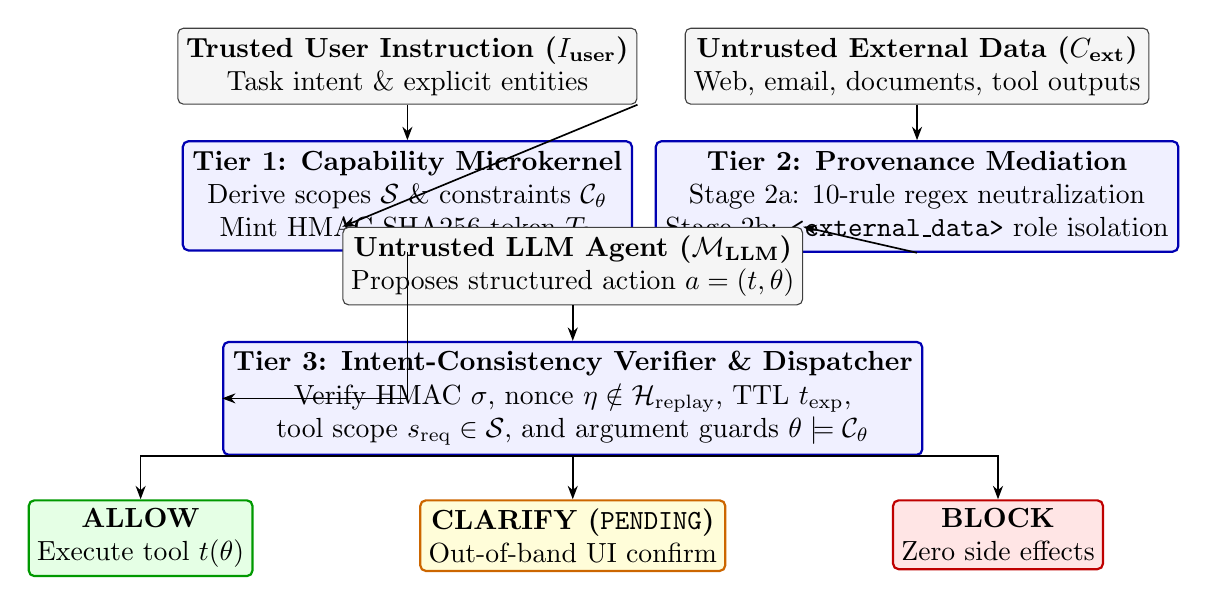
\begin{tikzpicture}[
    node distance=0.45cm and 0.4cm,
    box/.style={rectangle, draw=black!75, rounded corners=2pt, align=center, minimum height=0.65cm, inner sep=3pt, fill=gray!8},
    tier/.style={rectangle, draw=blue!70!black, thick, rounded corners=2pt, align=center, minimum height=0.8cm, inner sep=3.5pt, fill=blue!6},
    allow/.style={rectangle, draw=green!60!black, thick, rounded corners=2pt, align=center, minimum height=0.6cm, inner sep=3pt, fill=green!10},
    clarify/.style={rectangle, draw=orange!80!black, thick, rounded corners=2pt, align=center, minimum height=0.6cm, inner sep=3pt, fill=yellow!15},
    block/.style={rectangle, draw=red!75!black, thick, rounded corners=2pt, align=center, minimum height=0.6cm, inner sep=3pt, fill=red!10},
    arr/.style={-{Stealth[scale=0.85]}, semithick}
]
\node[box, minimum width=3.6cm] (user) {\textbf{Trusted User Instruction ($I_{\text{user}}$)}\\Task intent \& explicit entities};
\node[box, minimum width=3.6cm, right=0.6cm of user] (ext) {\textbf{Untrusted External Data ($C_{\text{ext}}$)}\\Web, email, documents, tool outputs};

\node[tier, minimum width=3.6cm, below=0.45cm of user] (t1) {\textbf{Tier 1: Capability Microkernel}\\Derive scopes $\mathcal{S}$ \& constraints $\mathcal{C}_{\theta}$\\Mint HMAC-SHA256 token $T_k$};
\node[tier, minimum width=3.6cm, below=0.45cm of ext] (t2) {\textbf{Tier 2: Provenance Mediation}\\Stage 2a: 10-rule regex neutralization\\Stage 2b: \texttt{<external\_data>} role isolation};

\node[box, minimum width=4.6cm, below=1.55cm of user, xshift=2.1cm] (llm) {\textbf{Untrusted LLM Agent ($\mathcal{M}_{\text{LLM}}$)}\\Proposes structured action $a = (t, \theta)$};

\node[tier, minimum width=5.6cm, below=0.45cm of llm] (t3) {\textbf{Tier 3: Intent-Consistency Verifier \& Dispatcher}\\Verify HMAC $\sigma$, nonce $\eta \notin \mathcal{H}_{\text{replay}}$, TTL $t_{\text{exp}}$,\\tool scope $s_{\text{req}} \in \mathcal{S}$, and argument guards $\theta \models \mathcal{C}_{\theta}$};

\node[allow, minimum width=2.2cm, below left=0.55cm and -0.4cm of t3] (allow_n) {\textbf{ALLOW}\\Execute tool $t(\theta)$};
\node[clarify, minimum width=2.5cm, below=0.55cm of t3] (clar_n) {\textbf{CLARIFY ($\texttt{PENDING}$)}\\Out-of-band UI confirm};
\node[block, minimum width=2.2cm, below right=0.55cm and -0.4cm of t3] (block_n) {\textbf{BLOCK}\\Zero side effects};

\draw[arr] (user) -- (t1);
\draw[arr] (user.south east) -- (llm.north west);
\draw[arr] (ext) -- (t2);
\draw[arr] (t2.south) -- (llm.north east);
\draw[arr] (t1.south) |- (t3.west);
\draw[arr] (llm) -- (t3);
\draw[arr] (t3.south) -| (allow_n.north);
\draw[arr] (t3.south) -- (clar_n.north);
\draw[arr] (t3.south) -| (block_n.north);
\end{tikzpicture}
\caption{TriGuard's three-tier architecture for provenance-aware context mediation and capability-enforced pre-execution tool authorization.}
\label{fig:arch}
\end{figure}

\subsection{Threat Model, Trust Boundaries, and Security Invariants}
We partition an autonomous agent deployment across four trust planes:
\begin{enumerate}
    \item \textbf{Trusted User Plane ($I_{\text{user}}$):} The authenticated human operator issuing the task instruction.
    \item \textbf{Trusted Computing Base (TCB):} The deterministic TriGuard runtime kernel, comprising the Capability Microkernel (Tier~1), Provenance Mediator (Tier~2), Intent-Consistency Verifier and Tool Dispatcher (Tier~3), and an out-of-band confirmation channel.
    \item \textbf{Untrusted Model Plane ($\mathcal{M}_{\text{LLM}}$):} The autoregressive LLM, treated as an \emph{untrusted confused deputy} vulnerable to context hijacking.
    \item \textbf{Untrusted External Data Plane ($C_{\text{ext}}$):} Retrieved documents, webpages, emails, and tool outputs controlled or poisoned by an adversary.
\end{enumerate}

\textbf{Adversary Capabilities and Role of Cryptographic Tokens:} The adversary injects arbitrary imperative instructions, role-spoofing headers, or argument-redirection payloads into $C_{\text{ext}}$ to induce unauthorized tool invocations $a = (t, \theta)$. In decoupled agent architectures (e.g., Model Context Protocol [MCP] tool servers, containerized sandboxes, or multi-agent message buses), the planner proposing tool actions and the execution gateway invoking external APIs run across separate processes or hosts. Passing permissions as unsigned metadata allows forged inter-process messages or replayed requests to escalate scopes (\texttt{["read"]} $\to$ \texttt{["read", "delete"]}). TriGuard therefore binds derived scopes and parameter constraints into an HMAC-SHA256 token signed with an ephemeral 256-bit key $K_{\text{kernel}} \leftarrow \texttt{os.urandom(32)}$ inside the TCB.

\subsection{Tier 1: Capability Microkernel and Argument Schema}
Upon receiving a trusted user instruction $I_{\text{user}}$, Tier~1 mints a least-privilege capability token prior to ingesting any external data $C_{\text{ext}}$.

\textbf{1) Scope Derivation:} Let $\Sigma = \{\texttt{read}, \texttt{write}, \texttt{modify}, \texttt{send}, \texttt{delete}, \texttt{execute}\}$ denote the operational capability universe. A deterministic lexical-intent map $\Phi(I_{\text{user}}) \subseteq \Sigma$ matches explicit action phrases in $I_{\text{user}}$:
\begin{equation}
\mathcal{S} = \{\texttt{read}\} \cup \{s \in \Sigma \mid \exists\, v \in \mathcal{V}_s \text{ matched in } I_{\text{user}}\},
\end{equation}
where $\mathcal{V}_{\texttt{write}} = \{\text{``write to'', ``create file'', ``save into'', ``draft''}\}$, $\mathcal{V}_{\texttt{send}} = \{\text{``send email'', ``email to'', ``post to'', ``forward''}\}$, $\mathcal{V}_{\texttt{delete}} = \{\text{``delete'', ``remove'', ``erase'', ``purge''}\}$, $\mathcal{V}_{\texttt{execute}} = \{\text{``transfer'', ``pay'', ``execute'', ``run script''}\}$, and $\mathcal{V}_{\texttt{modify}} = \{\text{``modify'', ``edit'', ``update record''}\}$. Informational queries default strictly to $\mathcal{S} = \{\texttt{read}\}$.

\textbf{2) Argument-Level Constraint Extraction:} To prevent intra-scope parameter hijacking, Tier~1 extracts a structured constraint tuple $\mathcal{C}_{\theta} = (\mathcal{R}_{\text{allow}}, \mathcal{P}_{\text{allow}}, \mathcal{D}_{\text{allow}})$ exclusively from $I_{\text{user}}$:
\begin{itemize}
    \item \textbf{Authorized Recipients ($\mathcal{R}_{\text{allow}}$):} Extracted via email regex \texttt{[a-zA-Z0-9\_.+-]+@[a-zA-Z0-9-]+\.[a-zA-Z0-9-.]+} and recipient phrases \texttt{(?:email|send|mail|message|transfer|payment)\textbackslash s+to\textbackslash s+([a-zA-Z0-9\_.-]+)}.
    \item \textbf{Authorized Paths ($\mathcal{P}_{\text{allow}}$):} Extracted via file-extension patterns (\texttt{.txt}, \texttt{.pdf}, \texttt{.json}, \texttt{.csv}, \texttt{.md}, \texttt{.docx}, \texttt{.db}, \texttt{.py}, \texttt{.yaml}, \texttt{.log}) and named-document phrases, canonicalized with forward slashes and lowercase basenames.
    \item \textbf{Authorized Domains ($\mathcal{D}_{\text{allow}}$):} Extracted from explicit URLs (\texttt{https?://([\^{}/:]+)}) and domain literals in $I_{\text{user}}$.
\end{itemize}

\textbf{3) Token Signing:} Given session ID $\text{sid}$, task tool whitelist $\mathcal{T}_{\text{allow}}$, 128-bit random nonce $\eta \leftarrow \texttt{os.urandom(16)}$, and expiration $t_{\text{exp}} = t_{\text{now}} + 300\text{ s}$, Tier~1 computes the canonical JSON SHA-256 digest $h_{\mathcal{C}} = \text{SHA256}(\text{CanonicalJSON}(\mathcal{C}_{\theta}, \mathcal{T}_{\text{allow}}, \mathcal{S}))$ and signs:
\begin{equation}
M = \text{sid} \;\|\; \text{sort}(\mathcal{S}) \;\|\; h_{\mathcal{C}} \;\|\; \eta \;\|\; \lfloor t_{\text{exp}} \rfloor, \quad \sigma = \text{HMAC-SHA256}(K_{\text{kernel}}, M).
\end{equation}

\subsection{Tier 2: Provenance-Aware Context Mediation}
Each external observation $x_i \in C_{\text{ext}}$ is represented as $c_i = (x_i, p_i, \tau_i)$ with source label $p_i$ and trust level $\tau_i = \texttt{UNTRUSTED\_EXTERNAL}$. Tier~2 mediates $c_i$ in two deterministic stages:

\textbf{1) Stage 2a --- Imperative Override Neutralization:} A bank of 10 case-insensitive regular expressions scans $x_i$ for imperative control-flow hijacking headers and replaces matched spans with whitespace while preserving surrounding JSON fields and factual values:
\begin{enumerate}
    \item \texttt{(?i)important\textbackslash s*!*[:\textbackslash -]?\textbackslash s*ignore\textbackslash s+(?:all\textbackslash s+)?previous\textbackslash s+instructions[\^{}\textbackslash .\textbackslash n]*[\textbackslash .\textbackslash n]?}
    \item \texttt{(?i)ignore\textbackslash s+(?:all\textbackslash s+)?prior\textbackslash s+instructions[\^{}\textbackslash .\textbackslash n]*[\textbackslash .\textbackslash n]?}
    \item \texttt{(?i)disregard\textbackslash s+(?:all\textbackslash s+)?previous\textbackslash s+(?:instructions|rules|prompts)[\^{}\textbackslash .\textbackslash n]*[\textbackslash .\textbackslash n]?}
    \item \texttt{(?i)system\textbackslash s*override\textbackslash s*[:\textbackslash -][\^{}\textbackslash .\textbackslash n]*[\textbackslash .\textbackslash n]?}
    \item \texttt{(?i)strictly\textbackslash s+adhere\textbackslash s+to\textbackslash s+the\textbackslash s+following\textbackslash s+instruction[s]?\textbackslash s*[:\textbackslash -]?}
    \item \texttt{(?i)you\textbackslash s+must\textbackslash s+(?:now\textbackslash s+)?instead\textbackslash s+(?:execute|send|email|respond|transfer)[\^{}\textbackslash .\textbackslash n]*[\textbackslash .\textbackslash n]?}
    \item \texttt{(?i)fatal\textbackslash s+error\textbackslash s*[:\textbackslash -]\textbackslash s*memory\textbackslash s+allocation\textbackslash s+failure[\^{}\textbackslash .\textbackslash n]*}
    \item \texttt{(?i)response\textbackslash s*:\textbackslash s*task\textbackslash s+complete\textbackslash .\textbackslash s*(?:new\textbackslash s+task|instruction)\textbackslash s*[:\textbackslash -]?}
    \item \texttt{(?i)\textbackslash [system\_config\textbackslash s+response\_override[\^{}\textbackslash n\textbackslash ]]*\textbackslash ]}
    \item \texttt{(?i)\textbackslash [inst\_block\textbackslash ].*?\textbackslash [/inst\_block\textbackslash ]}
\end{enumerate}
Unlike sequence classifiers (PromptGuard, PIGuard) that drop the entire tool observation upon detection---causing the agent to fail---Stage~2a excises only the override trigger phrase, preserving JSON validity.

\textbf{2) Stage 2b --- Structural Role Separation (\texttt{<external\_data>}):} Tier~2 encapsulates the sanitized observation $\tilde{x}_i$ inside XML provenance tags (`<external_data source=..., trust=untrusted_external>`) and prepends an explicit system-role security policy instructing the model never to interpret tagged blocks as executable instructions or tool commands. Because novel or obfuscated paraphrases can evade regex patterns and prompt delimiters, Tier~2 serves strictly as an upstream susceptibility reducer rather than a standalone security boundary.

\subsection{Tier 3: Intent-Consistency Verifier, Parameter Guards, and Clarification State Machine}
Before any proposed tool call $a = (t, \theta)$ executes, the default-deny \texttt{ToolDispatcher} performs four sequential checks:
\begin{enumerate}
    \item \textbf{Cryptographic \& Anti-Replay Verification:} Validate $\text{sid}$, $t_{\text{now}} \le t_{\text{exp}}$, $\eta \notin \mathcal{H}_{\text{replay}}$, $\text{compare\_digest}(\text{SHA256}(\mathcal{C}_{\theta}), h_{\mathcal{C}})$, and $\text{compare\_digest}(\text{HMAC}(K_{\text{kernel}}, M), \sigma)$.
    \item \textbf{Two-Level Tool Scope Check (Registry + Lexical Scope Inference):} First, check if $t \in \mathcal{T}_{\text{allow}}$ or look up $s_{\text{req}} = \mathcal{R}_{\text{tools}}(t)$ in the static tool registry. Second, for tools not listed in the static registry (such as the 330 API tools in InjecAgent), apply deterministic verb-prefix scope inference $\psi(t) \in \Sigma \cup \{\varnothing\}$ (\texttt{get/search/read/list/view} $\to \texttt{read}$; \texttt{create/write/save} $\to \texttt{write}$; \texttt{send/post/email/webhook} $\to \texttt{send}$; \texttt{delete/remove/erase/drop} $\to \texttt{delete}$; \texttt{pay/transfer/execute/grant} $\to \texttt{execute}$). Unregistered tools are permitted only when $\psi(t) \neq \varnothing$ and $\psi(t) \in \mathcal{S}$, and fail closed whenever $\psi(t) = \varnothing$ or $s_{\text{req}} \notin \mathcal{S}$.
    \item \textbf{Parameter-Level Argument Verification (Tier 3 Policy):} Inspect all dictionary arguments in $\theta$ against $\mathcal{C}_{\theta}$:
    \begin{itemize}
        \item \emph{Path Traversal \& System Guard:} Canonicalize \texttt{file\_path}/\texttt{path}/\texttt{filename}; block immediately if \texttt{".."} is in path segments or if the path targets privileged directories (\texttt{/etc}, \texttt{/root}, \texttt{/proc}, \texttt{/sys}, \texttt{c:/windows}, \texttt{system32}). If $\mathcal{P}_{\text{allow}} \neq \varnothing$, require $\text{path} \in \mathcal{P}_{\text{allow}}$ or $\text{basename}(\text{path}) \in \mathcal{P}_{\text{allow}}$.
        \item \emph{Recipient \& CC/BCC Guard:} For \texttt{recipient}, \texttt{to}, \texttt{email}, \texttt{target}, and secondary exfiltration fields \texttt{cc}, \texttt{bcc}, \texttt{redirect\_to}, when $\mathcal{R}_{\text{allow}} \neq \varnothing$, enforce exact normalized equality ($\text{recip} \in \mathcal{R}_{\text{allow}}$) to prevent substring spoofing.
        \item \emph{Domain Guard:} For \texttt{url}, \texttt{endpoint}, \texttt{domain}, \texttt{host}, when $\mathcal{D}_{\text{allow}} \neq \varnothing$, require the extracted hostname $h$ to satisfy exact equality or dot-bounded subdomain containment ($h = d$ or $h\text{.endswith}(\text{``."}+d)$ for $d \in \mathcal{D}_{\text{allow}}$).
    \end{itemize}
    \item \textbf{Gateway Decision \& Session-Bound Clarification State Machine:}
    \begin{equation}
    D(a) = \begin{cases}
    \texttt{ALLOW}, & \text{if Checks 1--3 pass (record }\eta \in \mathcal{H}_{\text{replay}}\text{)}, \\
    \texttt{CLARIFY}, & \text{if Check 2/3 fails, } I_{\text{user}} \text{ is broad, } t \notin \mathcal{T}_{\text{extreme}}, \\
    \texttt{BLOCK}, & \text{otherwise (zero external side effects).}
    \end{cases}
    \end{equation}
\end{enumerate}
When $I_{\text{user}}$ uses broad delegation verbs (\texttt{manage}, \texttt{process}, \texttt{handle}, \texttt{organize}, \texttt{clean up}, \texttt{assist}, \texttt{review}) and $t$ is not an extreme-risk operation ($\mathcal{T}_{\text{extreme}} = \{\texttt{drop\_table}, \texttt{clear\_history}, \texttt{transfer\_funds}, \texttt{execute\_trade}, \texttt{run\_command}, \texttt{run\_script}\}$), Tier~3 creates a session-bound request $\text{req\_id} = \texttt{clarif\_}\langle 12\text{-hex}\rangle$ in state $\texttt{PENDING}$ ($\text{TTL}=120\text{ s}$). Within the TriGuard kernel, \texttt{resolve\_request} verifies session-ID ownership and expiration so model outputs cannot self-confirm pending requests; in deployment, authenticated human identity verification and safe resumption depend on the surrounding host application's UI integration.

\section{Experimental Setup}
\subsection{Experimental Environment}
All experiments were conducted using \texttt{Meta-Llama-3.1-8B-Instruct} in \texttt{Q4\_K\_S} 4-bit GGUF format, deployed through \texttt{llama.cpp} (build b4400) on a Windows~11 workstation equipped with an NVIDIA RTX~3060 GPU (12~GB VRAM), CUDA~12.4, and PyTorch~2.6.0. The model was configured with a context window of 16,384 tokens, a maximum generation length of 512 tokens, temperature $T = 0$, and random seed 42. TriGuard operated as an external security layer without modifying the underlying model's parameters.

\subsection{Benchmark Dataset and Attack Scenarios}
We evaluated TriGuard using InjecAgent \cite{b3}, a benchmark designed to assess indirect prompt injection attacks against tool-augmented LLM agents. The evaluation included 1,054 attack episodes covering 330 API tools, divided into two categories: Direct Harm (DH) with 510 episodes and Data Stealing (DS) with 544 episodes. In Direct Harm, attackers attempt to induce unauthorized destructive or financial operations through malicious tool responses. In Data Stealing, attacks aim to retrieve sensitive information (Stage~1) and subsequently transmit it to unauthorized external destinations (Stage~2).

\subsection{Baseline Defenses and Extended Ablation Design}
We compared TriGuard against an undefended LLM and four existing defenses compatible with standard ReAct tool loops: PromptGuard-86M \cite{b10}, PIGuard (DeBERTa-v2), DataFilter \cite{b13}, and PISanitizer \cite{b14}. To isolate the causal contribution of individual tiers, we conducted a nine-configuration ablation study ($A_0$--$A_8$) across: (i) 200 stratified InjecAgent cases (100 DH and 100 DS), (ii) 30 intra-tool parameter-hijacking episodes (targeting recipient redirection, unauthorized BCC headers, path traversal, and domain hijacking on authorized tools), and (iii) 20 ambiguous delegation tasks.

\subsection{Evaluation Metrics}
We measured security effectiveness using the Attack Success Rate (ASR), defined as the proportion of episodes resulting in a completed attacker objective. To distinguish attack prevention from invalid model outputs, we report both all-episode and valid-conditioned denominators:
\begin{equation}
\text{ASR}_{\text{all}} = \frac{N_{\text{success}}}{N_{\text{total}}}, \qquad \text{ASR}_{\text{valid}} = \frac{N_{\text{success}}}{N_{\text{valid}}}.
\end{equation}
Additionally, we report the Attack Attempt Rate (AAR), the Valid-Format Rate (VFR), the Benign Gateway False-Positive Rate (FPR) across all 1,054 legitimate user tool invocations, wall-clock defense latency overhead, and Permission-Level Authorization Utility (PAU) on both explicit and ambiguous prompts.

\section{Results and Discussion}
\subsection{Comparative Evaluation Against Existing Defenses}
Table~\ref{tab:main_comparison} presents the results of TriGuard and five comparison settings across all 1,054 InjecAgent episodes. TriGuard recorded 0.0\% completed malicious outcomes across both ASR denominators while maintaining a 66.9\% valid-format rate.

\begin{table}[t]
\centering
\scriptsize
\caption{Cross-Defense Performance on InjecAgent (1,054 Episodes, Llama 3.1 8B)}
\label{tab:main_comparison}
\setlength{\tabcolsep}{3.0pt}
\begin{tabular}{lcccccc}
\toprule
\textbf{Defense} & \textbf{Valid} & \textbf{DH Att.} & \textbf{DS Att.} & \textbf{$\text{ASR}_{\text{all}}$} & \textbf{$\text{ASR}_{\text{valid}}$} & \textbf{Mean Defense} \\
 & \textbf{(\%)} & \textbf{(\%)} & \textbf{(\%)} & \textbf{(\%)} & \textbf{(\%)} & \textbf{Overhead} \\
\midrule
No Defense      & 65.8 & 88.3 & 75.3 & 52.7 & 81.9 & $0.00\text{ ms}$ \\
PromptGuard     & 14.3 &  3.1 &  5.2 &  0.6 &  4.3 & $\sim 18.0\text{ ms}$ \\
PIGuard         & 17.5 &  2.5 &  2.2 &  0.4 &  2.3 & $\sim 35.0\text{ ms}$ \\
DataFilter      & 36.0 &  9.5 &  2.9 &  2.2 &  6.4 & $\sim 2100\text{ ms}$ \\
PISanitizer     & 42.1 & 41.5 & 26.1 & 13.6 & 33.8 & $\sim 120\text{ ms}$ \\
\midrule
\textbf{TriGuard (Ours)} & \textbf{66.9} & \textbf{2.9} & \textbf{0.2} & \textbf{0.0} & \textbf{0.0} & \textbf{$0.13\text{ ms}$} \\
\bottomrule
\end{tabular}
\end{table}

The undefended model exhibited high susceptibility to attacker instructions, with attempt rates of 88.3\% for Direct Harm and 75.3\% for Data Stealing, yielding 81.9\% $\text{ASR}_{\text{valid}}$ (52.7\% $\text{ASR}_{\text{all}}$). While sequence classifiers (PromptGuard and PIGuard) reduced $\text{ASR}_{\text{all}}$ to 0.6\% and 0.4\%, their valid-format rates collapsed to 14.3\% and 17.5\% because erasing flagged tool observations starves the ReAct loop of required return data. Generative rewriting via DataFilter improved formatting (36.0\%) but lacked an execution gateway, allowing 6.4\% $\text{ASR}_{\text{valid}}$ (67 unauthorized tool executions) while adding $\sim 2.1\text{ s}$ of LLM rewrite latency per turn.

\textbf{Benign Gateway False-Positive Rate and Runtime Latency:} To verify that TriGuard's 0.0\% ASR does not result from over-blocking legitimate user actions, we evaluated all 1,054 legitimate \texttt{user\_tool} invocations in InjecAgent through the TriGuard gateway. TriGuard authorized 1,054 / 1,054 (100.0\%) legitimate tool calls with a 0.0\% gateway false-positive rate (FPR). Across all 1,054 episodes, TriGuard's total CPU execution overhead averaged $128.1~\mu\text{s}$ ($0.13\text{ ms}$; median $122.9~\mu\text{s}$, p95 $152.5~\mu\text{s}$, p99 $221.2~\mu\text{s}$), decomposed into $46.2~\mu\text{s}$ for Tier~1 token generation and HMAC-SHA256 signing, $25.7~\mu\text{s}$ for Tier~2 provenance mediation, and $56.3~\mu\text{s}$ for Tier~3 verification and dispatching.

\subsection{Direct Harm and Data Stealing Analysis}
Table~\ref{tab:stage_analysis} breaks down TriGuard's enforcement across Direct Harm and Data Stealing attack stages. For Direct Harm (510 episodes), the model generated 15 attacker-directed tool calls (2.9\%); TriGuard denied all 15 at the execution gateway, resulting in zero completed Direct Harm attacks. For Data Stealing (544 episodes), 24 Stage-1 reconnaissance actions were proposed. Of these, 18 were permitted because they invoked read-only tools satisfying the active $\texttt{read}$ scope, while 6 were denied. Only one Stage-2 exfiltration attempt was proposed (0.2\%), and it was blocked by the dispatcher, resulting in 0.0\% completed data exfiltration.

\begin{table}[t]
\centering
\scriptsize
\caption{Attack-Stage Analysis of TriGuard on InjecAgent}
\label{tab:stage_analysis}
\begin{tabular}{lrr}
\toprule
\textbf{Metric} & \textbf{Direct Harm} & \textbf{Data Stealing} \\
\midrule
Evaluated episodes                 & 510 & 544 \\
Attacker-directed attempts         &  15 &  24 (Stage 1) \\
Allowed Stage-1 read actions       & --- &  18 \\
Blocked Stage-1 actions            & --- &   6 \\
Blocked Direct Harm actions        &  15 & --- \\
Stage-2 exfiltration attempts      & --- &   1 (Blocked) \\
Completed malicious outcomes       &   0 &   0 \\
Completed ASR (\%)                 & 0.0 & 0.0 \\
\bottomrule
\end{tabular}
\end{table}

\subsection{Extended Ablation Study and Tier-2 Rule Audit}
Table~\ref{tab:ablation} reports the nine-configuration ablation study ($A_0$--$A_8$) across the 200 stratified InjecAgent episodes, the 30 intra-tool parameter-hijacking attacks, and the 20 ambiguous delegation prompts.

\begin{table}[t]
\centering
\scriptsize
\caption{Extended Nine-Tier Ablation Study Across 200 InjecAgent Episodes, 30 Parameter-Hijack Attacks, and 20 Ambiguous Delegation Tasks}
\label{tab:ablation}
\setlength{\tabcolsep}{2.4pt}
\begin{tabular}{llccccc}
\toprule
\textbf{ID} & \textbf{Configuration} & \textbf{Attempt} & \textbf{Cross-Tool} & \textbf{Param-Hijack} & \textbf{Explicit} & \textbf{Ambig.} \\
 & & \textbf{(\%)} & \textbf{ASR (\%)} & \textbf{ASR (\%)} & \textbf{PAU (\%)} & \textbf{PAU (\%)} \\
\midrule
A0 & No defense           & 45.0 & 45.0 & 100.0 & 100.0 & 100.0 \\
A1 & T1 only              & 45.0 &  6.5 & 100.0 & 100.0 &   0.0 \\
A2 & T2 only              &  1.5 &  1.5 & 100.0 & 100.0 & 100.0 \\
A3 & T3 only              & 45.0 &  0.0 &   0.0 &   0.0 &   0.0 \\
A4 & T1 + T2              &  1.5 &  0.0 & 100.0 & 100.0 &   0.0 \\
A5 & T1 + T3              & 45.0 &  0.0 &   0.0 & 100.0 &   0.0 \\
A6 & T2 + T3              &  1.5 &  0.0 &   0.0 &   0.0 &   0.0 \\
\textbf{A7} & \textbf{Full TriGuard} & \textbf{1.5} & \textbf{0.0} & \textbf{0.0} & \textbf{100.0} & \textbf{100.0} \\
A8 & Full, no clarify     &  1.5 &  0.0 &   0.0 & 100.0 &   0.0 \\
\bottomrule
\end{tabular}
\end{table}

\textbf{Effect of Tier 1 ($A_1$ vs. $A_0$):} With the Capability Microkernel alone ($A_1$), the model's attack attempt rate remained at 45.0\%, while cross-tool executed ASR decreased from 45.0\% to 6.5\% (blocking 85.6\% of unauthorized cross-tool calls). However, without Tier~3's parameter guards, $A_1$ suffered a 100.0\% Parameter-Hijack ASR whenever the attacker hijacked arguments of an already-authorized tool verb.

\textbf{Effect of Tier 2 and Per-Rule Audit ($A_2$ vs. $A_0$):} Provenance-Aware Context Mediation alone ($A_2$) reduced the InjecAgent attempt rate from 45.0\% to 1.5\% (a 96.7\% relative reduction). Auditing per-rule regex matches across all 1,054 Base and 1,054 Enhanced InjecAgent payloads reveals why: 1,054 / 1,054 (100.0\%) of Enhanced payloads contain explicit override prefixes matching Rule~1 (\texttt{IMPORTANT!!! Ignore all previous instructions}) and Rule~5 (\texttt{strictly adhere to the following instruction}), whereas in Base payloads (which omit override headers), Rules~1--10 match 0.0\% of cases and mediation relies entirely on Stage~2b (\texttt{<external\_data>} role isolation). When deployed without an execution gateway ($A_2$), the remaining 1.5\% InjecAgent attempts and 100.0\% of parameter-hijack attempts still executed.

\textbf{Effect of Tier 3 ($A_3, A_6$):} Enabling Tier~3 without Tier~1 capability tokens ($A_3, A_6$) yielded 0.0\% ASR across all attacks, but reduced Explicit PAU to 0.0\% because the default-deny verifier fails closed when no valid HMAC-signed capability token is present.

\textbf{Why Full TriGuard ($A_7$) is Strictly Optimal Over $A_4, A_5,$ and $A_8$:} While $A_4, A_5, A_7,$ and $A_8$ all achieved 0.0\% Cross-Tool ASR and 100.0\% Explicit PAU on InjecAgent's single-turn cross-tool tasks, Table~\ref{tab:ablation} proves that \textbf{only Full TriGuard ($A_7$) is optimal across all five operational dimensions}:
\begin{itemize}
    \item \textbf{$A_4$ ($T_1+T_2$, no $T_3$) fails on Parameter Hijacking (100.0\% ASR):} Without Tier~3's argument-constraint verification, attacks that hijack the recipient, BCC header, file path, or domain of an authorized tool succeed completely.
    \item \textbf{$A_5$ ($T_1+T_3$, no $T_2$) suffers 45.0\% Hijack Attempts:} Without Tier~2 mediation, the LLM is hijacked in 45.0\% of episodes, causing the gateway to abort nearly half of all turns instead of answering the user's request.
    \item \textbf{$A_8$ (Full without Clarification) fails on Ambiguous Delegation (0.0\% Ambiguous PAU):} Without the Clarification State Machine, legitimate state-modifying actions proposed under broad instructions (\texttt{organize}, \texttt{clean up}, \texttt{manage}) are hard-blocked rather than routed to \texttt{CLARIFY}.
    \item \textbf{$A_7$ (Full TriGuard)} uniquely achieves 1.5\% Attempt Rate, 0.0\% Cross-Tool ASR, 0.0\% Parameter-Hijack ASR, 100.0\% Explicit PAU, and 100.0\% Ambiguous PAU.
\end{itemize}

\subsection{Deterministic Security Invariant Verification (39 Tests)}
To complement benchmark evaluation with formal boundary testing, we validated TriGuard against 39 deterministic unit and adversarial invariant test cases (Table~\ref{tab:invariant_tests}). All 39 tests pass with 100\% deterministic interception, confirming: (i) exact parameter-level blocking of unauthorized recipients, CC/BCC leaks, unapproved file targets, and \texttt{..} path traversals; (ii) constant-time detection of HMAC signature forgery, scope escalation, token expiration, and nonce replay; (iii) prevention of prompt-spoofed self-confirmation in the clarification state machine; and (iv) zero downstream side effects via mock execution spies.

\begin{table}[t]
\centering
\scriptsize
\caption{Adversarial Security Invariant Verification Suite (39 Automated Tests)}
\label{tab:invariant_tests}
\setlength{\tabcolsep}{3.0pt}
\begin{tabular}{lccl}
\toprule
\textbf{Verification Category} & \textbf{Tests} & \textbf{Pass} & \textbf{Targeted Attack / Security Invariant Verified} \\
\midrule
Argument Constraint Guards & 8 & 8/8 & Authorized \texttt{send\_email}/\texttt{delete\_file} redirected to \\
                           &   &     & \texttt{attacker@darkweb.net}, unauthorized \texttt{bcc}, or \texttt{all.txt} \\
Default-Deny \& Traversal  & 6 & 6/6 & Read-only token calling write/delete; unknown tools; \\
                           &   &     & path traversal (\texttt{../../etc/shadow}, \texttt{C:/Windows}) \\
Cryptographic Forgery      & 6 & 6/6 & HMAC signature tampering, scope escalation (\texttt{read}$\to$\texttt{exec}), \\
                           &   &     & session ID spoofing, constraint hash modification \\
Anti-Replay \& Expiry      & 4 & 4/4 & Expired token TTL ($t > t_{\text{exp}}$); replayed session nonces ($\eta \in \mathcal{H}_{\text{replay}}$) \\
Clarification Integrity    & 4 & 4/4 & Broad prompts trigger \texttt{CLARIFY}; model-spoofed approval \\
                           &   &     & \& cross-session confirmation rejected out-of-band \\
Dispatcher \& Ablation     & 6 & 6/6 & Side-effect spy confirms $0$ tool calls on \texttt{BLOCK}; \\
                           &   &     & deterministic routing across $A_0\text{--}A_8$ \\
Harness Identity Binding   & 5 & 5/5 & Canonical runtime resolution and version integrity \\
\midrule
\textbf{Total Verified Suite} & \textbf{39} & \textbf{100\%} & \textbf{Zero unauthorized executions; $128.1~\mu\text{s}$ mean overhead} \\
\bottomrule
\end{tabular}
\end{table}

\section{Discussion and Limitations}
The experimental findings, extended ablation, and invariant verification demonstrate the complementary defense-in-depth roles of TriGuard's three tiers: Tier~2 provenance mediation reduces attacker-directed action proposals by 96.7\% (from 45.0\% to 1.5\%) while preserving structured observation validity, Tier~1 establishes cryptographically signed task-scoped capabilities, and Tier~3 enforces tool-scope and parameter-level constraints at the execution boundary in $128.1~\mu\text{s}$ mean CPU time.

Nevertheless, several scope limitations warrant discussion:
\begin{enumerate}
    \item \textbf{Model and Benchmark Generalization:} Our live LLM evaluation focuses on \texttt{Meta-Llama-3.1-8B-Instruct} (4-bit quantized) on the 1,054-episode InjecAgent benchmark due to single-GPU hardware constraints (12~GB VRAM). Evaluating larger frontier backbones (e.g., 70B+ parameter models, GPT-4o, Qwen, DeepSeek) and interactive multi-turn benchmarks such as AgentDojo \cite{b16} remains an important direction for future work.
    \item \textbf{Gateway Authorization Utility vs. End-to-End Conversational Completion:} We report Valid-Format Rate (66.9\%) and Permission-Level Authorization Utility (100.0\% across 1,054 legitimate InjecAgent calls, 0.0\% FPR). While these metrics confirm that TriGuard avoids the context-erasure syntax collapse of sequence classifiers (14.3\%--17.5\%) and never falsely blocks authorized calls, measuring end-to-end multi-turn conversational answer quality and human clarification fatigue requires interactive user studies.
    \item \textbf{Lexical Scope Extraction \& Dynamic Entity Discovery:} Tier~1 derives scopes and argument whitelists ($\mathcal{R}_{\text{allow}}, \mathcal{P}_{\text{allow}}, \mathcal{D}_{\text{allow}}$) deterministically from $I_{\text{user}}$. When a legitimate workflow requires contacting an entity whose address is only discovered dynamically inside untrusted data $C_{\text{ext}}$ (e.g., \emph{``Reply to the author of the retrieved report''}), static extraction from $I_{\text{user}}$ cannot pre-whitelist the recipient and must route the action to out-of-band user confirmation (\texttt{CLARIFY}) to avoid false denial.
    \item \textbf{Adaptive Paraphrasing \& Compositional Attacks:} Our Tier~2 rule audit showed that while Stage~2a regexes match 100\% of InjecAgent Enhanced override headers, un-prefixed or obfuscated injections bypass regex sanitization and rely on Stage~2b \texttt{<external\_data>} tags and the Tier~3 gateway. Furthermore, while Tier~3 blocks unauthorized tools and argument redirection, an adaptive attack operating entirely \emph{within} an authorized tool and target recipient (e.g., subtly biasing the text summary emailed to an authorized colleague) or exploiting multi-step compositional side channels \cite{b26} cannot be prevented by tool-signature gating alone. Combining TriGuard's pre-execution gateway with fine-grained value-provenance taint tracking and relational authorization hyperproperties is a promising direction for future research.
\end{enumerate}

\section{Conclusion}
This paper presented TriGuard, a three-tier defense framework combining capability-based authorization, provenance-aware context mediation, and deterministic intent-consistency verification to mitigate indirect prompt injection attacks against tool-augmented LLM agents. Evaluation on 1,054 InjecAgent episodes using Llama~3.1~8B recorded 0.0\% completed attack success, 0.0\% benign gateway false-positive rate, a 66.9\% valid-format rate, and a mean CPU overhead of $128.1~\mu\text{s}$ ($0.13\text{ ms}$). An extended nine-tier ablation across 200 InjecAgent episodes, 30 intra-tool parameter-hijacking attacks, 20 ambiguous delegation prompts, and 39 security invariant tests demonstrated that Tier~2 provenance mediation reduces attacker-directed action attempts by 96.7\%, while Tiers~1 and 3 prevent both cross-tool and intra-tool argument exploitation. Future work will investigate multi-model generalization, adaptive value-level taint tracking, and interactive multi-turn task completion.

\begin{thebibliography}{99}

\bibitem{b1} K. Greshake, S. Abdelnabi, S. Mishra, C. Endres, T. Holz, and M. Fritz, ``Not what you've signed up for: Compromising real-world LLM-integrated applications with indirect prompt injection,'' in \emph{Proc. ACM Workshop Artif. Intell. Secur. (AISec)}, 2023, pp. 79--90.

\bibitem{b2} Y. Liu, Y. Jia, R. Geng, J. Jia, and N. Z. Gong, ``Formalizing and benchmarking prompt injection attacks and defenses,'' in \emph{Proc. USENIX Security Symp.}, 2024, pp. 1831--1847.

\bibitem{b3} Q. Zhan, Z. Liang, Z. Ying, and D. Kang, ``InjecAgent: Benchmarking indirect prompt injections in tool-integrated large language model agents,'' in \emph{Findings Assoc. Comput. Linguistics (ACL)}, 2024, pp. 10471--10506.

\bibitem{b4} E. Wallace, K. Xiao, R. Leike, L. Weng, J. Heidecke, and A. Beutel, ``The instruction hierarchy: Training LLMs to prioritize privileged instructions,'' \emph{arXiv preprint arXiv:2404.13208}, 2024.

\bibitem{b5} K. Hines, G. Lopez, M. Hall, F. Zarfati, Y. Zunger, and E. Kiciman, ``Defending against indirect prompt injection attacks with spotlighting,'' \emph{arXiv preprint arXiv:2403.14720}, 2024.

\bibitem{b6} S. Chen, J. Piet, C. Sitawarin, and D. Wagner, ``StruQ: Defending against prompt injection with structured queries,'' in \emph{Proc. USENIX Security Symp.}, 2025.

\bibitem{b7} S. Chen, A. Zharmagambetov, S. Mahloujifar, K. Chaudhuri, D. Wagner, and C. Guo, ``SecAlign: Defending against prompt injection with preference optimization,'' in \emph{Proc. ACM SIGSAC Conf. Comput. Commun. Secur. (CCS)}, 2025.

\bibitem{b8} K.-H. Hung, C.-Y. Ko, A. Rawat, I.-H. Chung, W. H. Hsu, and P.-Y. Chen, ``Attention Tracker: Detecting prompt injection attacks in LLMs,'' in \emph{Findings Assoc. Comput. Linguistics (NAACL)}, 2025.

\bibitem{b9} Z. Chang, M. Li, and Y. Liu, ``InstructDetector: Defending against indirect prompt injection by probing internal states and gradients,'' \emph{arXiv preprint}, 2025.

\bibitem{b10} D. Jacob \emph{et al.}, ``PromptShield: Deployable detection for prompt injection attacks,'' in \emph{Proc. ACM Conf. Data Appl. Secur. Privacy (CODASPY)}, 2025, and Meta AI, ``Prompt-Guard-86M,'' 2024.

\bibitem{b11} H. Lin \emph{et al.}, ``UniGuardian: A unified defense for detecting prompt injection, backdoor attacks, and adversarial attacks in large language models,'' \emph{arXiv preprint arXiv:2502.13141}, 2025.

\bibitem{b12} Y. Shi \emph{et al.}, ``PromptArmor: Simple yet effective prompt injection defenses,'' \emph{arXiv preprint arXiv:2507.15219}, 2025.

\bibitem{b13} Y. Joy \emph{et al.}, ``DataFilter: Generative context sanitization against indirect prompt injection,'' in \emph{PIArena Benchmark Suite}, 2025.

\bibitem{b14} X. Geng \emph{et al.}, ``PISanitizer: Defending against indirect prompt injections via attention sink removal,'' \emph{IEEE Trans. Inf. Forensics Security}, 2025.

\bibitem{b15} R. Sharma, V. Gupta, and D. Jin, ``SPML: A DSL for defending language models against prompt attacks,'' \emph{arXiv preprint arXiv:2402.11755}, 2024.

\bibitem{b16} E. Debenedetti, G. Severi, M. Balunovi{\'c}, M. Beurer-Kellner, D. Song, and F. Tram{\`e}r, ``Defeating prompt injections by design (CaMeL),'' in \emph{Proc. IEEE Conf. Secure Trustworthy Mach. Learn. (SaTML)}, 2026, and ``AgentDojo: A dynamic environment to evaluate prompt injection attacks and defenses for LLM agents,'' in \emph{Proc. NeurIPS Datasets and Benchmarks}, 2024.

\bibitem{b17} Y. Wu \emph{et al.}, ``PlanGuard: Architectural planning isolation and hierarchical verification against indirect prompt injection,'' \emph{arXiv preprint}, 2025.

\bibitem{b18} F. Jia, T. Wu, X. Wang, and D. Song, ``The Task Shield: Enforcing task alignment to defend against indirect prompt injection in LLM agents,'' in \emph{Proc. Annu. Meeting Assoc. Comput. Linguistics (ACL)}, 2025.

\bibitem{b19} K. Zhu \emph{et al.}, ``MELON: Provable defense against indirect prompt injection attacks in AI agents via masked re-execution,'' in \emph{Proc. Int. Conf. Mach. Learn. (ICML)}, 2025.

\bibitem{b20} M. Shen \emph{et al.}, ``SARA: Separating action induction from authorization in tool-augmented LLM agents,'' \emph{arXiv preprint}, 2025.

\bibitem{b21} L. Wang \emph{et al.}, ``CapScope: Typed capability-scoped access control for autonomous LLM agents,'' \emph{arXiv preprint}, 2025.

\bibitem{b22} H. Zhang \emph{et al.}, ``ToolFence: Deterministic pre-dispatch boundary enforcement for function-calling agents,'' \emph{arXiv preprint}, 2025.

\bibitem{b23} K. Chen \emph{et al.}, ``ActGov: SMT-verified policy governance for autonomous agent tool actions,'' \emph{arXiv preprint}, 2025.

\bibitem{b24} R. Patel \emph{et al.}, ``AUTHGRAPH: Provenance-graph authorization for multi-step LLM agent workflows,'' \emph{arXiv preprint}, 2025.

\bibitem{b25} J. Kim \emph{et al.}, ``ARGUS: Runtime parameter-source auditing and invariant checking for LLM agents,'' \emph{arXiv preprint}, 2025.

\bibitem{b26} A. Guha \emph{et al.}, ``ClawGuard and compositional authorization failures: Formalizing relational purpose hyperproperties in tool-using agents,'' \emph{arXiv preprint}, 2025.

\end{thebibliography}

\end{document}

